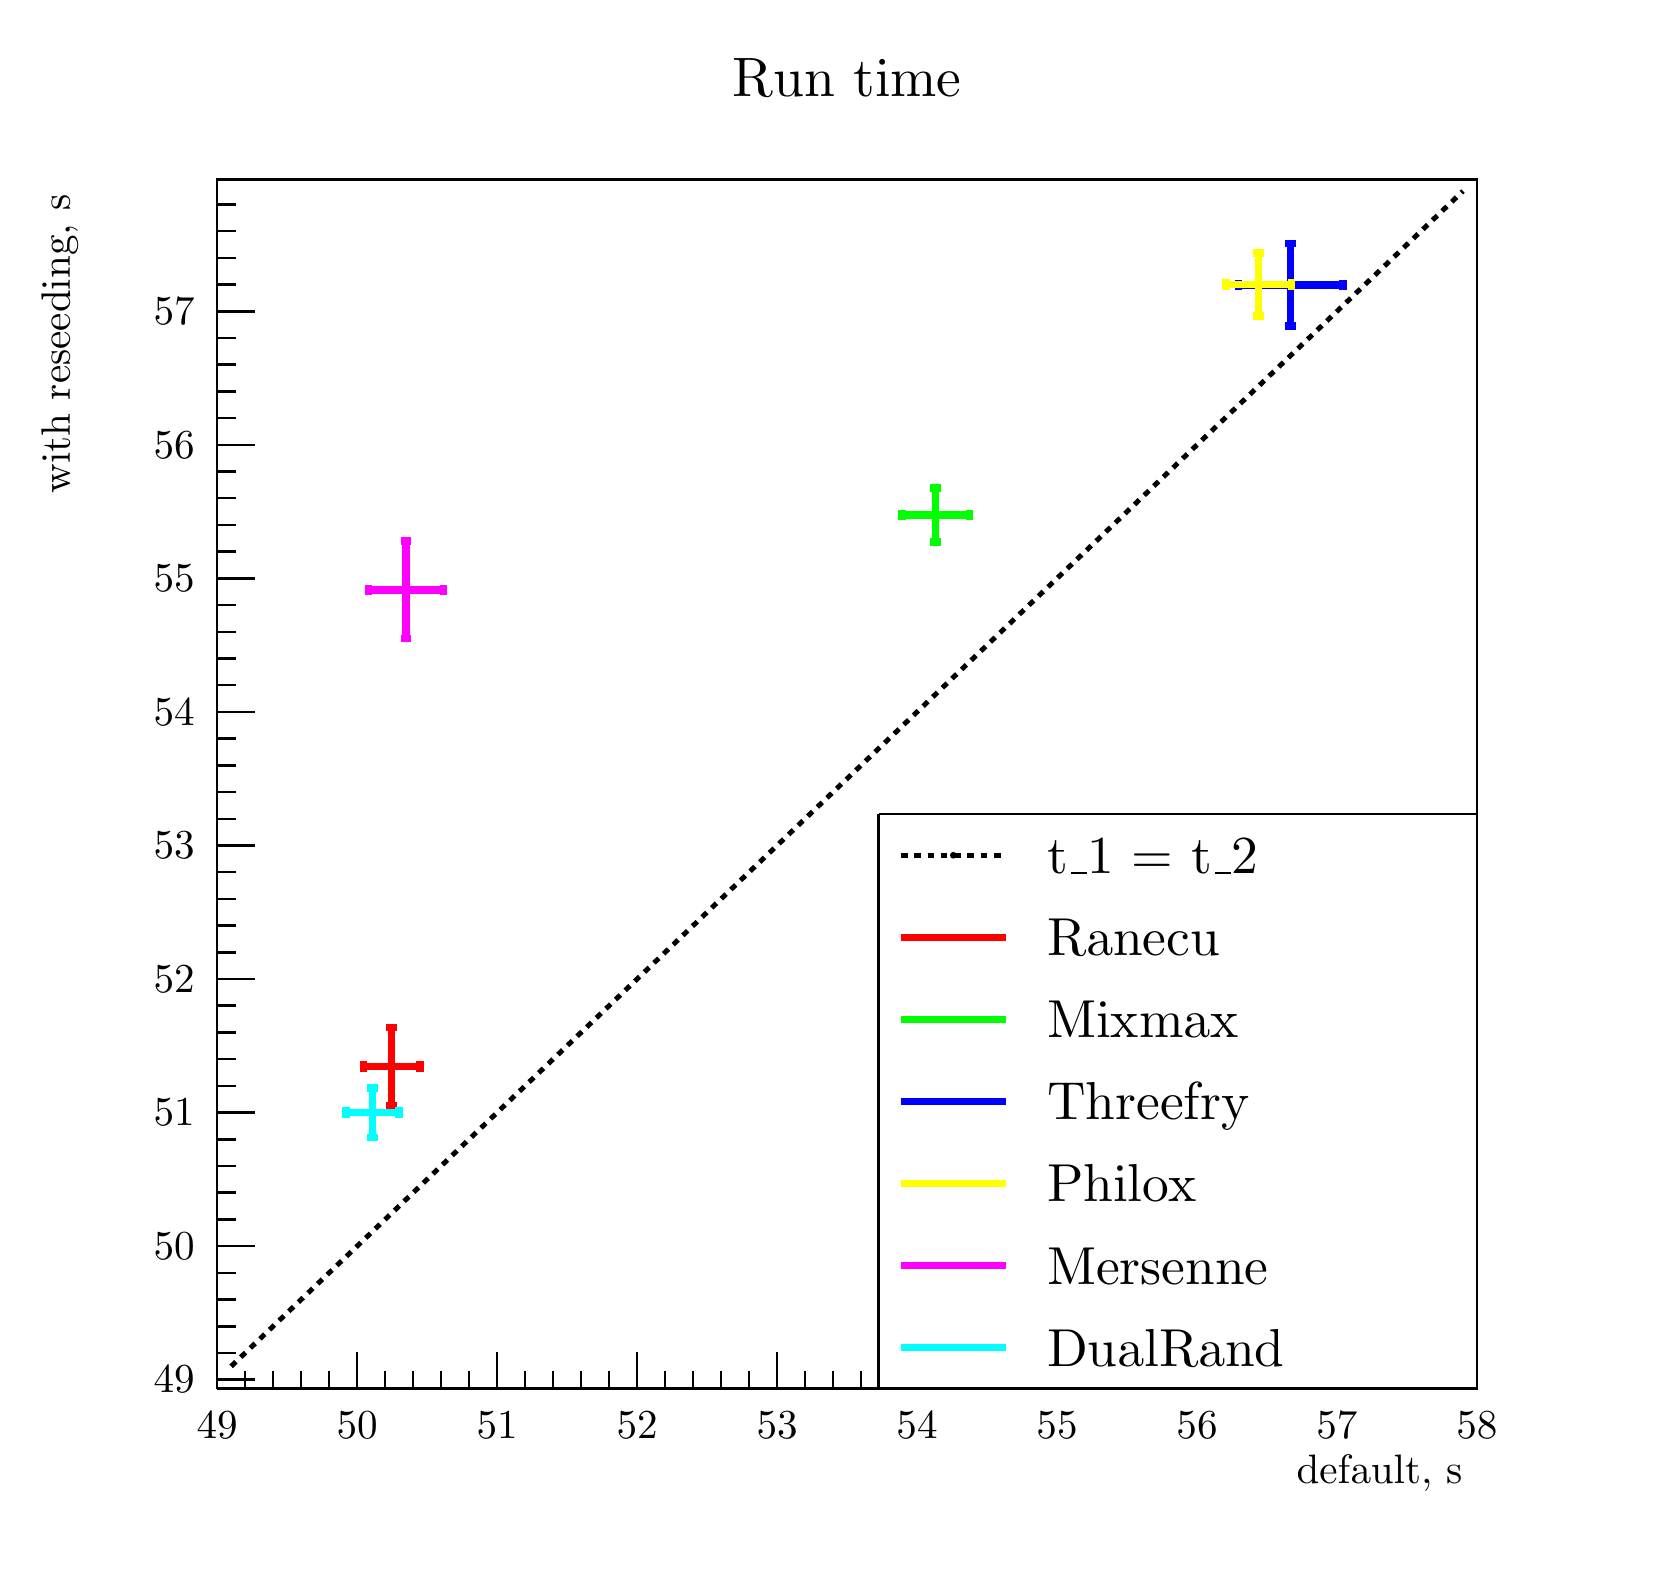
\begin{tikzpicture}
\pgfdeclareplotmark{cross} {
\pgfpathmoveto{\pgfpoint{-0.3\pgfplotmarksize}{\pgfplotmarksize}}
\pgfpathlineto{\pgfpoint{+0.3\pgfplotmarksize}{\pgfplotmarksize}}
\pgfpathlineto{\pgfpoint{+0.3\pgfplotmarksize}{0.3\pgfplotmarksize}}
\pgfpathlineto{\pgfpoint{+1\pgfplotmarksize}{0.3\pgfplotmarksize}}
\pgfpathlineto{\pgfpoint{+1\pgfplotmarksize}{-0.3\pgfplotmarksize}}
\pgfpathlineto{\pgfpoint{+0.3\pgfplotmarksize}{-0.3\pgfplotmarksize}}
\pgfpathlineto{\pgfpoint{+0.3\pgfplotmarksize}{-1.\pgfplotmarksize}}
\pgfpathlineto{\pgfpoint{-0.3\pgfplotmarksize}{-1.\pgfplotmarksize}}
\pgfpathlineto{\pgfpoint{-0.3\pgfplotmarksize}{-0.3\pgfplotmarksize}}
\pgfpathlineto{\pgfpoint{-1.\pgfplotmarksize}{-0.3\pgfplotmarksize}}
\pgfpathlineto{\pgfpoint{-1.\pgfplotmarksize}{0.3\pgfplotmarksize}}
\pgfpathlineto{\pgfpoint{-0.3\pgfplotmarksize}{0.3\pgfplotmarksize}}
\pgfpathclose
\pgfusepathqstroke
}
\pgfdeclareplotmark{cross*} {
\pgfpathmoveto{\pgfpoint{-0.3\pgfplotmarksize}{\pgfplotmarksize}}
\pgfpathlineto{\pgfpoint{+0.3\pgfplotmarksize}{\pgfplotmarksize}}
\pgfpathlineto{\pgfpoint{+0.3\pgfplotmarksize}{0.3\pgfplotmarksize}}
\pgfpathlineto{\pgfpoint{+1\pgfplotmarksize}{0.3\pgfplotmarksize}}
\pgfpathlineto{\pgfpoint{+1\pgfplotmarksize}{-0.3\pgfplotmarksize}}
\pgfpathlineto{\pgfpoint{+0.3\pgfplotmarksize}{-0.3\pgfplotmarksize}}
\pgfpathlineto{\pgfpoint{+0.3\pgfplotmarksize}{-1.\pgfplotmarksize}}
\pgfpathlineto{\pgfpoint{-0.3\pgfplotmarksize}{-1.\pgfplotmarksize}}
\pgfpathlineto{\pgfpoint{-0.3\pgfplotmarksize}{-0.3\pgfplotmarksize}}
\pgfpathlineto{\pgfpoint{-1.\pgfplotmarksize}{-0.3\pgfplotmarksize}}
\pgfpathlineto{\pgfpoint{-1.\pgfplotmarksize}{0.3\pgfplotmarksize}}
\pgfpathlineto{\pgfpoint{-0.3\pgfplotmarksize}{0.3\pgfplotmarksize}}
\pgfpathclose
\pgfusepathqfillstroke
}
\pgfdeclareplotmark{newstar} {
\pgfpathmoveto{\pgfqpoint{0pt}{\pgfplotmarksize}}
\pgfpathlineto{\pgfqpointpolar{44}{0.5\pgfplotmarksize}}
\pgfpathlineto{\pgfqpointpolar{18}{\pgfplotmarksize}}
\pgfpathlineto{\pgfqpointpolar{-20}{0.5\pgfplotmarksize}}
\pgfpathlineto{\pgfqpointpolar{-54}{\pgfplotmarksize}}
\pgfpathlineto{\pgfqpointpolar{-90}{0.5\pgfplotmarksize}}
\pgfpathlineto{\pgfqpointpolar{234}{\pgfplotmarksize}}
\pgfpathlineto{\pgfqpointpolar{198}{0.5\pgfplotmarksize}}
\pgfpathlineto{\pgfqpointpolar{162}{\pgfplotmarksize}}
\pgfpathlineto{\pgfqpointpolar{134}{0.5\pgfplotmarksize}}
\pgfpathclose
\pgfusepathqstroke
}
\pgfdeclareplotmark{newstar*} {
\pgfpathmoveto{\pgfqpoint{0pt}{\pgfplotmarksize}}
\pgfpathlineto{\pgfqpointpolar{44}{0.5\pgfplotmarksize}}
\pgfpathlineto{\pgfqpointpolar{18}{\pgfplotmarksize}}
\pgfpathlineto{\pgfqpointpolar{-20}{0.5\pgfplotmarksize}}
\pgfpathlineto{\pgfqpointpolar{-54}{\pgfplotmarksize}}
\pgfpathlineto{\pgfqpointpolar{-90}{0.5\pgfplotmarksize}}
\pgfpathlineto{\pgfqpointpolar{234}{\pgfplotmarksize}}
\pgfpathlineto{\pgfqpointpolar{198}{0.5\pgfplotmarksize}}
\pgfpathlineto{\pgfqpointpolar{162}{\pgfplotmarksize}}
\pgfpathlineto{\pgfqpointpolar{134}{0.5\pgfplotmarksize}}
\pgfpathclose
\pgfusepathqfillstroke
}
\definecolor{c}{rgb}{1,1,1};
\draw [color=c, fill=c] (0,0) rectangle (20,19.1973);
\draw [color=c, fill=c] (2,1.91973) rectangle (18,17.2776);
\definecolor{c}{rgb}{0,0,0};
\draw [c,line width=0.9] (2,1.91973) -- (2,17.2776) -- (18,17.2776) -- (18,1.91973) -- (2,1.91973);
\definecolor{c}{rgb}{1,1,1};
\draw [color=c, fill=c] (2,1.91973) rectangle (18,17.2776);
\definecolor{c}{rgb}{0,0,0};
\draw [c,line width=0.9] (2,1.91973) -- (2,17.2776) -- (18,17.2776) -- (18,1.91973) -- (2,1.91973);
\draw [c,dash pattern=on 2.40pt off 2.40pt ,line width=1.8] (2.17778,2.20336) -- (2.53333,2.54258) -- (2.88889,2.8818) -- (3.24444,3.22101) -- (3.6,3.56023) -- (3.95556,3.89945) -- (4.31111,4.23867) -- (4.66667,4.57788) -- (5.02222,4.9171) --
 (5.37778,5.25632) -- (5.73333,5.59554) -- (6.08889,5.93475) -- (6.44444,6.27397) -- (6.8,6.61319) -- (7.15556,6.9524) -- (7.51111,7.29162) -- (7.86667,7.63084) -- (8.22222,7.97006) -- (8.57778,8.30927) -- (8.93333,8.64849) -- (9.28889,8.98771) --
 (9.64444,9.32693) -- (10,9.66614) -- (10.3556,10.0054) -- (10.7111,10.3446) -- (11.0667,10.6838) -- (11.4222,11.023) -- (11.7778,11.3622) -- (12.1333,11.7014) -- (12.4889,12.0407) -- (12.8444,12.3799) -- (13.2,12.7191) -- (13.5556,13.0583) --
 (13.9111,13.3975) -- (14.2667,13.7368) -- (14.6222,14.076) -- (14.9778,14.4152) -- (15.3333,14.7544) -- (15.6889,15.0936) -- (16.0444,15.4328) -- (16.4,15.7721) -- (16.7556,16.1113) -- (17.1111,16.4505) -- (17.4667,16.7897) -- (17.8222,17.1289);
\draw [c,line width=0.9] (2,1.91973) -- (18,1.91973);
\draw [c,line width=0.9] (2,2.38047) -- (2,1.91973);
\draw [c,line width=0.9] (2.35556,2.1501) -- (2.35556,1.91973);
\draw [c,line width=0.9] (2.71111,2.1501) -- (2.71111,1.91973);
\draw [c,line width=0.9] (3.06667,2.1501) -- (3.06667,1.91973);
\draw [c,line width=0.9] (3.42222,2.1501) -- (3.42222,1.91973);
\draw [c,line width=0.9] (3.77778,2.38047) -- (3.77778,1.91973);
\draw [c,line width=0.9] (4.13333,2.1501) -- (4.13333,1.91973);
\draw [c,line width=0.9] (4.48889,2.1501) -- (4.48889,1.91973);
\draw [c,line width=0.9] (4.84444,2.1501) -- (4.84444,1.91973);
\draw [c,line width=0.9] (5.2,2.1501) -- (5.2,1.91973);
\draw [c,line width=0.9] (5.55556,2.38047) -- (5.55556,1.91973);
\draw [c,line width=0.9] (5.91111,2.1501) -- (5.91111,1.91973);
\draw [c,line width=0.9] (6.26667,2.1501) -- (6.26667,1.91973);
\draw [c,line width=0.9] (6.62222,2.1501) -- (6.62222,1.91973);
\draw [c,line width=0.9] (6.97778,2.1501) -- (6.97778,1.91973);
\draw [c,line width=0.9] (7.33333,2.38047) -- (7.33333,1.91973);
\draw [c,line width=0.9] (7.68889,2.1501) -- (7.68889,1.91973);
\draw [c,line width=0.9] (8.04444,2.1501) -- (8.04444,1.91973);
\draw [c,line width=0.9] (8.4,2.1501) -- (8.4,1.91973);
\draw [c,line width=0.9] (8.75556,2.1501) -- (8.75556,1.91973);
\draw [c,line width=0.9] (9.11111,2.38047) -- (9.11111,1.91973);
\draw [c,line width=0.9] (9.46667,2.1501) -- (9.46667,1.91973);
\draw [c,line width=0.9] (9.82222,2.1501) -- (9.82222,1.91973);
\draw [c,line width=0.9] (10.1778,2.1501) -- (10.1778,1.91973);
\draw [c,line width=0.9] (10.5333,2.1501) -- (10.5333,1.91973);
\draw [c,line width=0.9] (10.8889,2.38047) -- (10.8889,1.91973);
\draw [c,line width=0.9] (11.2444,2.1501) -- (11.2444,1.91973);
\draw [c,line width=0.9] (11.6,2.1501) -- (11.6,1.91973);
\draw [c,line width=0.9] (11.9556,2.1501) -- (11.9556,1.91973);
\draw [c,line width=0.9] (12.3111,2.1501) -- (12.3111,1.91973);
\draw [c,line width=0.9] (12.6667,2.38047) -- (12.6667,1.91973);
\draw [c,line width=0.9] (13.0222,2.1501) -- (13.0222,1.91973);
\draw [c,line width=0.9] (13.3778,2.1501) -- (13.3778,1.91973);
\draw [c,line width=0.9] (13.7333,2.1501) -- (13.7333,1.91973);
\draw [c,line width=0.9] (14.0889,2.1501) -- (14.0889,1.91973);
\draw [c,line width=0.9] (14.4444,2.38047) -- (14.4444,1.91973);
\draw [c,line width=0.9] (14.8,2.1501) -- (14.8,1.91973);
\draw [c,line width=0.9] (15.1556,2.1501) -- (15.1556,1.91973);
\draw [c,line width=0.9] (15.5111,2.1501) -- (15.5111,1.91973);
\draw [c,line width=0.9] (15.8667,2.1501) -- (15.8667,1.91973);
\draw [c,line width=0.9] (16.2222,2.38047) -- (16.2222,1.91973);
\draw [c,line width=0.9] (16.5778,2.1501) -- (16.5778,1.91973);
\draw [c,line width=0.9] (16.9333,2.1501) -- (16.9333,1.91973);
\draw [c,line width=0.9] (17.2889,2.1501) -- (17.2889,1.91973);
\draw [c,line width=0.9] (17.6444,2.1501) -- (17.6444,1.91973);
\draw [c,line width=0.9] (18,2.38047) -- (18,1.91973);
\draw [anchor=base] (2,1.28622) node[scale=1.4856, color=c, rotate=0]{49};
\draw [anchor=base] (3.77778,1.28622) node[scale=1.4856, color=c, rotate=0]{50};
\draw [anchor=base] (5.55556,1.28622) node[scale=1.4856, color=c, rotate=0]{51};
\draw [anchor=base] (7.33333,1.28622) node[scale=1.4856, color=c, rotate=0]{52};
\draw [anchor=base] (9.11111,1.28622) node[scale=1.4856, color=c, rotate=0]{53};
\draw [anchor=base] (10.8889,1.28622) node[scale=1.4856, color=c, rotate=0]{54};
\draw [anchor=base] (12.6667,1.28622) node[scale=1.4856, color=c, rotate=0]{55};
\draw [anchor=base] (14.4444,1.28622) node[scale=1.4856, color=c, rotate=0]{56};
\draw [anchor=base] (16.2222,1.28622) node[scale=1.4856, color=c, rotate=0]{57};
\draw [anchor=base] (18,1.28622) node[scale=1.4856, color=c, rotate=0]{58};
\draw [anchor= east] (18,0.844682) node[scale=1.4856, color=c, rotate=0]{default, s};
\draw [c,line width=0.9] (2,1.91973) -- (2,17.2776);
\draw [c,line width=0.9] (2.48,2.03375) -- (2,2.03375);
\draw [c,line width=0.9] (2.24,2.37297) -- (2,2.37297);
\draw [c,line width=0.9] (2.24,2.71219) -- (2,2.71219);
\draw [c,line width=0.9] (2.24,3.05141) -- (2,3.05141);
\draw [c,line width=0.9] (2.24,3.39062) -- (2,3.39062);
\draw [c,line width=0.9] (2.48,3.72984) -- (2,3.72984);
\draw [c,line width=0.9] (2.24,4.06906) -- (2,4.06906);
\draw [c,line width=0.9] (2.24,4.40827) -- (2,4.40827);
\draw [c,line width=0.9] (2.24,4.74749) -- (2,4.74749);
\draw [c,line width=0.9] (2.24,5.08671) -- (2,5.08671);
\draw [c,line width=0.9] (2.48,5.42593) -- (2,5.42593);
\draw [c,line width=0.9] (2.24,5.76514) -- (2,5.76514);
\draw [c,line width=0.9] (2.24,6.10436) -- (2,6.10436);
\draw [c,line width=0.9] (2.24,6.44358) -- (2,6.44358);
\draw [c,line width=0.9] (2.24,6.7828) -- (2,6.7828);
\draw [c,line width=0.9] (2.48,7.12201) -- (2,7.12201);
\draw [c,line width=0.9] (2.24,7.46123) -- (2,7.46123);
\draw [c,line width=0.9] (2.24,7.80045) -- (2,7.80045);
\draw [c,line width=0.9] (2.24,8.13967) -- (2,8.13967);
\draw [c,line width=0.9] (2.24,8.47888) -- (2,8.47888);
\draw [c,line width=0.9] (2.48,8.8181) -- (2,8.8181);
\draw [c,line width=0.9] (2.24,9.15732) -- (2,9.15732);
\draw [c,line width=0.9] (2.24,9.49654) -- (2,9.49654);
\draw [c,line width=0.9] (2.24,9.83575) -- (2,9.83575);
\draw [c,line width=0.9] (2.24,10.175) -- (2,10.175);
\draw [c,line width=0.9] (2.48,10.5142) -- (2,10.5142);
\draw [c,line width=0.9] (2.24,10.8534) -- (2,10.8534);
\draw [c,line width=0.9] (2.24,11.1926) -- (2,11.1926);
\draw [c,line width=0.9] (2.24,11.5318) -- (2,11.5318);
\draw [c,line width=0.9] (2.24,11.8711) -- (2,11.8711);
\draw [c,line width=0.9] (2.48,12.2103) -- (2,12.2103);
\draw [c,line width=0.9] (2.24,12.5495) -- (2,12.5495);
\draw [c,line width=0.9] (2.24,12.8887) -- (2,12.8887);
\draw [c,line width=0.9] (2.24,13.2279) -- (2,13.2279);
\draw [c,line width=0.9] (2.24,13.5671) -- (2,13.5671);
\draw [c,line width=0.9] (2.48,13.9064) -- (2,13.9064);
\draw [c,line width=0.9] (2.24,14.2456) -- (2,14.2456);
\draw [c,line width=0.9] (2.24,14.5848) -- (2,14.5848);
\draw [c,line width=0.9] (2.24,14.924) -- (2,14.924);
\draw [c,line width=0.9] (2.24,15.2632) -- (2,15.2632);
\draw [c,line width=0.9] (2.48,15.6024) -- (2,15.6024);
\draw [c,line width=0.9] (2.48,2.03375) -- (2,2.03375);
\draw [c,line width=0.9] (2.48,15.6024) -- (2,15.6024);
\draw [c,line width=0.9] (2.24,15.9417) -- (2,15.9417);
\draw [c,line width=0.9] (2.24,16.2809) -- (2,16.2809);
\draw [c,line width=0.9] (2.24,16.6201) -- (2,16.6201);
\draw [c,line width=0.9] (2.24,16.9593) -- (2,16.9593);
\draw [anchor= east] (1.9,2.03375) node[scale=1.4856, color=c, rotate=0]{49};
\draw [anchor= east] (1.9,3.72984) node[scale=1.4856, color=c, rotate=0]{50};
\draw [anchor= east] (1.9,5.42593) node[scale=1.4856, color=c, rotate=0]{51};
\draw [anchor= east] (1.9,7.12201) node[scale=1.4856, color=c, rotate=0]{52};
\draw [anchor= east] (1.9,8.8181) node[scale=1.4856, color=c, rotate=0]{53};
\draw [anchor= east] (1.9,10.5142) node[scale=1.4856, color=c, rotate=0]{54};
\draw [anchor= east] (1.9,12.2103) node[scale=1.4856, color=c, rotate=0]{55};
\draw [anchor= east] (1.9,13.9064) node[scale=1.4856, color=c, rotate=0]{56};
\draw [anchor= east] (1.9,15.6024) node[scale=1.4856, color=c, rotate=0]{57};
\draw [anchor= east] (0.0,17.2776) node[scale=1.4856, color=c, rotate=90]{with reseeding, s};
\definecolor{c}{rgb}{1,0,0};
\draw [c,line width=2.7] (4.21511,6.00938) -- (3.856,6.00938);
\draw [c,line width=2.7] (3.856,5.94249) -- (3.856,6.07627);
\draw [c,line width=2.7] (4.21511,6.00938) -- (4.57422,6.00938);
\draw [c,line width=2.7] (4.57422,5.94249) -- (4.57422,6.07627);
\draw [c,line width=2.7] (4.21511,6.00938) -- (4.21511,6.50464);
\draw [c,line width=2.7] (4.14822,6.50464) -- (4.282,6.50464);
\draw [c,line width=2.7] (4.21511,6.00938) -- (4.21511,5.51412);
\draw [c,line width=2.7] (4.14822,5.51412) -- (4.282,5.51412);
\foreach \P in {(4.21511,6.00938)}{\draw[mark options={color=c,fill=c},mark size=2.402402pt,mark=*,mark size=1pt] plot coordinates {\P};}
\definecolor{c}{rgb}{0,1,0};
\draw [c,line width=2.7] (11.1253,13.0125) -- (10.6987,13.0125);
\draw [c,line width=2.7] (10.6987,12.9456) -- (10.6987,13.0794);
\draw [c,line width=2.7] (11.1253,13.0125) -- (11.552,13.0125);
\draw [c,line width=2.7] (11.552,12.9456) -- (11.552,13.0794);
\draw [c,line width=2.7] (11.1253,13.0125) -- (11.1253,13.3551);
\draw [c,line width=2.7] (11.0584,13.3551) -- (11.1922,13.3551);
\draw [c,line width=2.7] (11.1253,13.0125) -- (11.1253,12.6699);
\draw [c,line width=2.7] (11.0584,12.6699) -- (11.1922,12.6699);
\foreach \P in {(11.1253,13.0125)}{\draw[mark options={color=c,fill=c},mark size=2.402402pt,mark=*,mark size=1pt] plot coordinates {\P};}
\definecolor{c}{rgb}{0,0,1};
\draw [c,line width=2.7] (15.6338,15.9383) -- (14.9707,15.9383);
\draw [c,line width=2.7] (14.9707,15.8714) -- (14.9707,16.0052);
\draw [c,line width=2.7] (15.6338,15.9383) -- (16.2969,15.9383);
\draw [c,line width=2.7] (16.2969,15.8714) -- (16.2969,16.0052);
\draw [c,line width=2.7] (15.6338,15.9383) -- (15.6338,16.4641);
\draw [c,line width=2.7] (15.5669,16.4641) -- (15.7007,16.4641);
\draw [c,line width=2.7] (15.6338,15.9383) -- (15.6338,15.4125);
\draw [c,line width=2.7] (15.5669,15.4125) -- (15.7007,15.4125);
\foreach \P in {(15.6338,15.9383)}{\draw[mark options={color=c,fill=c},mark size=2.402402pt,mark=*,mark size=1pt] plot coordinates {\P};}
\definecolor{c}{rgb}{1,1,0};
\draw [c,line width=2.7] (15.2284,15.9434) -- (14.8124,15.9434);
\draw [c,line width=2.7] (14.8124,15.8765) -- (14.8124,16.0103);
\draw [c,line width=2.7] (15.2284,15.9434) -- (15.6444,15.9434);
\draw [c,line width=2.7] (15.6444,15.8765) -- (15.6444,16.0103);
\draw [c,line width=2.7] (15.2284,15.9434) -- (15.2284,16.3419);
\draw [c,line width=2.7] (15.1616,16.3419) -- (15.2953,16.3419);
\draw [c,line width=2.7] (15.2284,15.9434) -- (15.2284,15.5448);
\draw [c,line width=2.7] (15.1616,15.5448) -- (15.2953,15.5448);
\foreach \P in {(15.2284,15.9434)}{\draw[mark options={color=c,fill=c},mark size=2.402402pt,mark=*,mark size=1pt] plot coordinates {\P};}
\definecolor{c}{rgb}{1,0,1};
\draw [c,line width=2.7] (4.39822,12.0644) -- (3.92178,12.0644);
\draw [c,line width=2.7] (3.92178,11.9975) -- (3.92178,12.1313);
\draw [c,line width=2.7] (4.39822,12.0644) -- (4.87467,12.0644);
\draw [c,line width=2.7] (4.87467,11.9975) -- (4.87467,12.1313);
\draw [c,line width=2.7] (4.39822,12.0644) -- (4.39822,12.6852);
\draw [c,line width=2.7] (4.33133,12.6852) -- (4.46511,12.6852);
\draw [c,line width=2.7] (4.39822,12.0644) -- (4.39822,11.4436);
\draw [c,line width=2.7] (4.33133,11.4436) -- (4.46511,11.4436);
\foreach \P in {(4.39822,12.0644)}{\draw[mark options={color=c,fill=c},mark size=2.402402pt,mark=*,mark size=1pt] plot coordinates {\P};}
\definecolor{c}{rgb}{0,1,1};
\draw [c,line width=2.7] (3.97333,5.42593) -- (3.63556,5.42593);
\draw [c,line width=2.7] (3.63556,5.35904) -- (3.63556,5.49282);
\draw [c,line width=2.7] (3.97333,5.42593) -- (4.31111,5.42593);
\draw [c,line width=2.7] (4.31111,5.35904) -- (4.31111,5.49282);
\draw [c,line width=2.7] (3.97333,5.42593) -- (3.97333,5.7397);
\draw [c,line width=2.7] (3.90644,5.7397) -- (4.04022,5.7397);
\draw [c,line width=2.7] (3.97333,5.42593) -- (3.97333,5.11215);
\draw [c,line width=2.7] (3.90644,5.11215) -- (4.04022,5.11215);
\foreach \P in {(3.97333,5.42593)}{\draw[mark options={color=c,fill=c},mark size=2.402402pt,mark=*,mark size=1pt] plot coordinates {\P};}
\definecolor{c}{rgb}{1,1,1};
\draw [color=c, fill=c] (10.4,1.91973) rectangle (18,9.21472);
\definecolor{c}{rgb}{0,0,0};
\draw [c,line width=0.9] (10.4,1.91973) -- (18,1.91973);
\draw [c,line width=0.9] (18,1.91973) -- (18,9.21472);
\draw [c,line width=0.9] (18,9.21472) -- (10.4,9.21472);
\draw [c,line width=0.9] (10.4,9.21472) -- (10.4,1.91973);
\draw [anchor=base west] (12.3,8.45916) node[scale=1.93128, color=c, rotate=0]{t\_1 = t\_2};
\definecolor{c}{rgb}{1,1,1};
\draw [c] (10.685,8.3289) -- (12.015,8.3289) -- (12.015,9.05839) -- (10.685,9.05839);
\definecolor{c}{rgb}{0,0,0};
\draw [c,dash pattern=on 2.40pt off 2.40pt ,line width=1.8] (10.685,8.69365) -- (12.015,8.69365);
\foreach \P in {(11.35,8.69365)}{\draw[mark options={color=c,fill=c},mark size=2.402402pt,mark=*,mark size=1pt] plot coordinates {\P};}
\draw [anchor=base west] (12.3,7.41702) node[scale=1.93128, color=c, rotate=0]{Ranecu};
\definecolor{c}{rgb}{1,1,1};
\draw [c, fill=c] (10.685,7.28676) -- (12.015,7.28676) -- (12.015,8.01625) -- (10.685,8.01625);
\definecolor{c}{rgb}{1,0,0};
\draw [c,line width=2.7] (10.685,7.6515) -- (12.015,7.6515);
\foreach \P in {(11.35,7.6515)}{\draw[mark options={color=c,fill=c},mark size=2.402402pt,mark=*,mark size=1pt] plot coordinates {\P};}
\definecolor{c}{rgb}{0,0,0};
\draw [anchor=base west] (12.3,6.37488) node[scale=1.93128, color=c, rotate=0]{Mixmax};
\definecolor{c}{rgb}{1,1,1};
\draw [c, fill=c] (10.685,6.24462) -- (12.015,6.24462) -- (12.015,6.97411) -- (10.685,6.97411);
\definecolor{c}{rgb}{0,1,0};
\draw [c,line width=2.7] (10.685,6.60936) -- (12.015,6.60936);
\foreach \P in {(11.35,6.60936)}{\draw[mark options={color=c,fill=c},mark size=2.402402pt,mark=*,mark size=1pt] plot coordinates {\P};}
\definecolor{c}{rgb}{0,0,0};
\draw [anchor=base west] (12.3,5.33274) node[scale=1.93128, color=c, rotate=0]{Threefry};
\definecolor{c}{rgb}{1,1,1};
\draw [c, fill=c] (10.685,5.20248) -- (12.015,5.20248) -- (12.015,5.93197) -- (10.685,5.93197);
\definecolor{c}{rgb}{0,0,1};
\draw [c,line width=2.7] (10.685,5.56722) -- (12.015,5.56722);
\foreach \P in {(11.35,5.56722)}{\draw[mark options={color=c,fill=c},mark size=2.402402pt,mark=*,mark size=1pt] plot coordinates {\P};}
\definecolor{c}{rgb}{0,0,0};
\draw [anchor=base west] (12.3,4.2906) node[scale=1.93128, color=c, rotate=0]{Philox};
\definecolor{c}{rgb}{1,1,1};
\draw [c, fill=c] (10.685,4.16033) -- (12.015,4.16033) -- (12.015,4.88983) -- (10.685,4.88983);
\definecolor{c}{rgb}{1,1,0};
\draw [c,line width=2.7] (10.685,4.52508) -- (12.015,4.52508);
\foreach \P in {(11.35,4.52508)}{\draw[mark options={color=c,fill=c},mark size=2.402402pt,mark=*,mark size=1pt] plot coordinates {\P};}
\definecolor{c}{rgb}{0,0,0};
\draw [anchor=base west] (12.3,3.24846) node[scale=1.93128, color=c, rotate=0]{Mersenne};
\definecolor{c}{rgb}{1,1,1};
\draw [c, fill=c] (10.685,3.11819) -- (12.015,3.11819) -- (12.015,3.84769) -- (10.685,3.84769);
\definecolor{c}{rgb}{1,0,1};
\draw [c,line width=2.7] (10.685,3.48294) -- (12.015,3.48294);
\foreach \P in {(11.35,3.48294)}{\draw[mark options={color=c,fill=c},mark size=2.402402pt,mark=*,mark size=1pt] plot coordinates {\P};}
\definecolor{c}{rgb}{0,0,0};
\draw [anchor=base west] (12.3,2.20632) node[scale=1.93128, color=c, rotate=0]{DualRand};
\definecolor{c}{rgb}{1,1,1};
\draw [c, fill=c] (10.685,2.07605) -- (12.015,2.07605) -- (12.015,2.80555) -- (10.685,2.80555);
\definecolor{c}{rgb}{0,1,1};
\draw [c,line width=2.7] (10.685,2.4408) -- (12.015,2.4408);
\foreach \P in {(11.35,2.4408)}{\draw[mark options={color=c,fill=c},mark size=2.402402pt,mark=*,mark size=1pt] plot coordinates {\P};}
\definecolor{c}{rgb}{0,0,0};
\draw (10,18.5734) node[scale=2.00556, color=c, rotate=0]{Run time};
\end{tikzpicture}
